\documentclass{article}

\title{A \LaTeX Workshop \\ for All Skill Levels}
\author{D. Zack G.}
\date{\today}

\usepackage{hyperref}
\usepackage{amsmath, amssymb, amsthm}
\usepackage{graphicx}
\usepackage{parskip}
\usepackage{float}

\newcommand{\RR}[1]{\mathbb{R}^{#1}}

\begin{document}

\maketitle
\newpage
\tableofcontents
\newpage

\section{Introduction}
    Document content goes here!
    
    We can't just say y = mx + b.
    
    Use inline math with $y = mx + b$.
    
    Equation math is $$y = mx + b$$

\section{Content}
	\subsection{Mathematics}
        \subsubsection{Inline Math}
        	Example: $f(x)=ax^2 + c_1$
        \subsubsection{Block-Level Math}
        	Example: $$ \sum_{i=0}^\infty i = -\frac{1}{12} $$
        	
\section{More Content}
    More unrelated text
		
    $\sum_{i=0}^\infty i = -\frac{1}{12}$
    
    The function $f: \RR{n} \rightarrow \RR{n}$ is \textit{continuous} if
    $$\lim_{n\rightarrow\infty} x_n = x \Rightarrow \lim_{n\rightarrow\infty} f(x_n) = f(x)$$
    
$$
M=
  \left[ {
      \begin{array}{ccc}
       1 & \alpha_1 & \alpha_1^2 \\
       1 & \alpha_2 & \alpha_2^2 \\
       1 & \alpha_3 & \alpha_3^2 \\
      \end{array}
  } \right]
$$
    
$\Box, \blacksquare$


\section{Even More Content}

\begin{figure}[H]
    \centering
    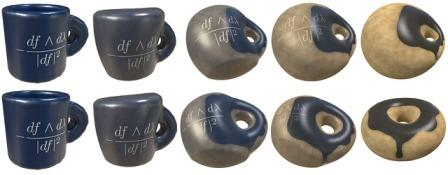
\includegraphics[width=4cm]{homotopy}
    \label{fig:myname}
    \caption{Delicious!}
\end{figure}    

\begin{equation} \label{eu_eqn}
    e^{\pi i} + 1 = 0
\end{equation}

See Equation~\ref{eu_eqn} 

\begin{equation*}
	\boxed{e^{\pi i} + 1 = 0}
\end{equation*}

\end{document}